% Many thanks to Andrew West for writing most of this file
% Main LaTeX file for CIS400/401 Project Proposal Specification
%
% Once built and in PDF form this document outlines the format of a
% project proposal. However, in raw (.tex) form, we also try to
% comment on some basic LaTeX technique. This is not intended to be a
% LaTeX tutorial, instead just (1) a use-case thereof, and (2) a
% template for your own writing.

% Ordinarily we'd begin by specifying some broad document properties
% like font-size, page-size, margins, etc. -- We have done this (and
% much more) for you by creating a 'style file', which the
% 'documentclass' command references.
\documentclass{sig-alternate}
 
% These 'usepackage' commands are a way of importing additional LaTeX
% styles and formattings that aren't part of the 'standard library'
\usepackage{mdwlist}
\usepackage{url}
\usepackage{tabularx}
\usepackage{tikz}
\usetikzlibrary{shapes,arrows}
\usepackage[export]{adjustbox}
\usepackage{lipsum,adjustbox}
\usepackage{listings}% http://ctan.org/pkg/listings
\lstset{
  basicstyle=\ttfamily,
  mathescape
}\begin{document} 

% We setup the parameters to our title header before 'making' it. Note
% that your proposals should have actual titles, not the generic one
% we have here.
\title{Verification of System FC in Coq}
\subtitle{Dept. of CIS - Senior Design 2014-2015\thanks{Advisors: Stephanie Weirich (sweirich@cis.upenn.edu), Richard Eisenberg (eir@cis.upenn.edu).}}
\numberofauthors{4}
\author{
  Tiernan Garsys \\ \email{tgarsys@seas.upenn.edu} \\ Univ. of Pennsylvania \\ Philadelphia, PA\\\\
  Lucas Pe\~{n}a \\ \email{lpena@seas.upenn.edu} \\ Univ. of Pennsylvania \\ Philadelphia, PA
  \and
  Tayler Mandel \\ \email{tmandel@seas.upenn.edu} \\ Univ. of Pennsylvania \\ Philadelphia, PA\\\\
  Noam Zilberstein \\ \email{noamz@seas.upenn.edu} \\ Univ. of Pennsylvania \\ Philadelphia, PA
}
\date{}
\maketitle

% Next we write out our abstract -- generally a two paragraph maximum,
% executive summary of the motivation and contributions of the work.
\begin{abstract}
\textit{
Haskell is a statically-typed functional programming language that is commonly used for the robust compile-time guarantees provided by its type system. Despite this usage, the type safety of Haskell has not been mechanically proven; it may be possible to write Haskell programs that type-check at compile-time but fall into an inconsistent state at runtime. Many safety critical systems such as flight controllers, self driving cars, and missile controllers are powered by software. If the type systems underlying this code are not verified, then the code itself is unsafe.
}

\textit{
This work approaches this problem by verifying System FC, the formalization of the core language of the Haskell compiler. It presents a mechanized proof for a large subset of System FC using the Coq Proof Assistant.  The type system of System FC is the basis for the type system of Haskell, so the results translate directly into safety guarantees at the program level.
}
\end{abstract}

% Then we proceed into the body of the report itself. The effect of
% the 'section' command is obvious, but also notice 'label'. Its good
% practice to label every (sub)-section, graph, equation etc. -- this
% gives us a way to dynamically reference it later in the text via the
% 'ref' command, e.g., instead of writing `Section 1', you can write
% `Section~\ref{sec:intro}', which is useful if the section number
% changes.

\section{Introduction}
\label{sec:intro}


Content content content

\section{Background}
\label{sec:background}

\subsection{Haskell}
\label{sec:background-haskell}

Haskell is a functional programming language originally released in 1990. Haskell is a statically-typed language; the types of all expressions and variables are determined at compile-time via either type inference or explicit type annotations by the programmer. Haskell is strongly-typed, meaning that the usage of values in identifier declarations and functions must be consistent with the statically-declared types of these functions; Haskell will not implicitly convert values from one type to another in order to satisfy the static typing of the program. Haskell is also a purely-functional language; a function defined in Haskell is guaranteed not to have side-effects such as I/O or the mutation of data structures in the running environment unless this is explictly allowed by the programmer. 

The strong static typing of Haskell is attractive because it allows the programmer to make certain guarantees about the properties of his or her program at compilation, rather than runtime. Such guarantees include the guarantee that a function is never called with an invalid input type, or the guarantee that a function defines a behavior for null inputs. By determining these properties at compile-time, one can rule out entire classes of errors prior to ever running the program.

These advantages are founded on the believed type safety of Haskell. Type safety in a programming language refers to its resilience to type errors at runtime. In the context of a statically-typed language such as Haskell, type safety requires ensuring that the guarantees of behavior made at compile-time are preserved during program execution. Given type safety, one can be sure that the program does not exhibit undefined behavior (such as segmentation faults) during execution.

\subsection{GHC Core}
\label{sec:background-ghc-core}

The Glasgow Haskell Compiler, or GHC, is an optimizing compiler used to generate native executables from Haskell code. As with most compilers, GHC compiles programs in multiple phases, translating the source between various intermediate representations. These phases of compilation are outlined in Figure~\ref{fig:desgar}. Whereas a surface language, such as Haskell, is structured to be easy for humans to work with, these intermediate representations (also known as {\em core languages}) are designed to be easy for a compiler to modify and optimize.

In the first phase of compilation, Haskell code is type-checked and then converted into a desugared intermediate language called GHC Core. The conversion from Haskell to GHC Core involves adding explicit type annotations to all values (which, in Haskell, can be omitted by the programmer and subsequently inferred when type-checking), adding explicit type parameters to type declarations with polymorphic types, and assigning all identifiers globally-unique names. Once converted, GHC performs optimizations on the resulting GHC Core code before passing the program on to later stages of compilation.

\begin{figure}[h!]
  \centering
  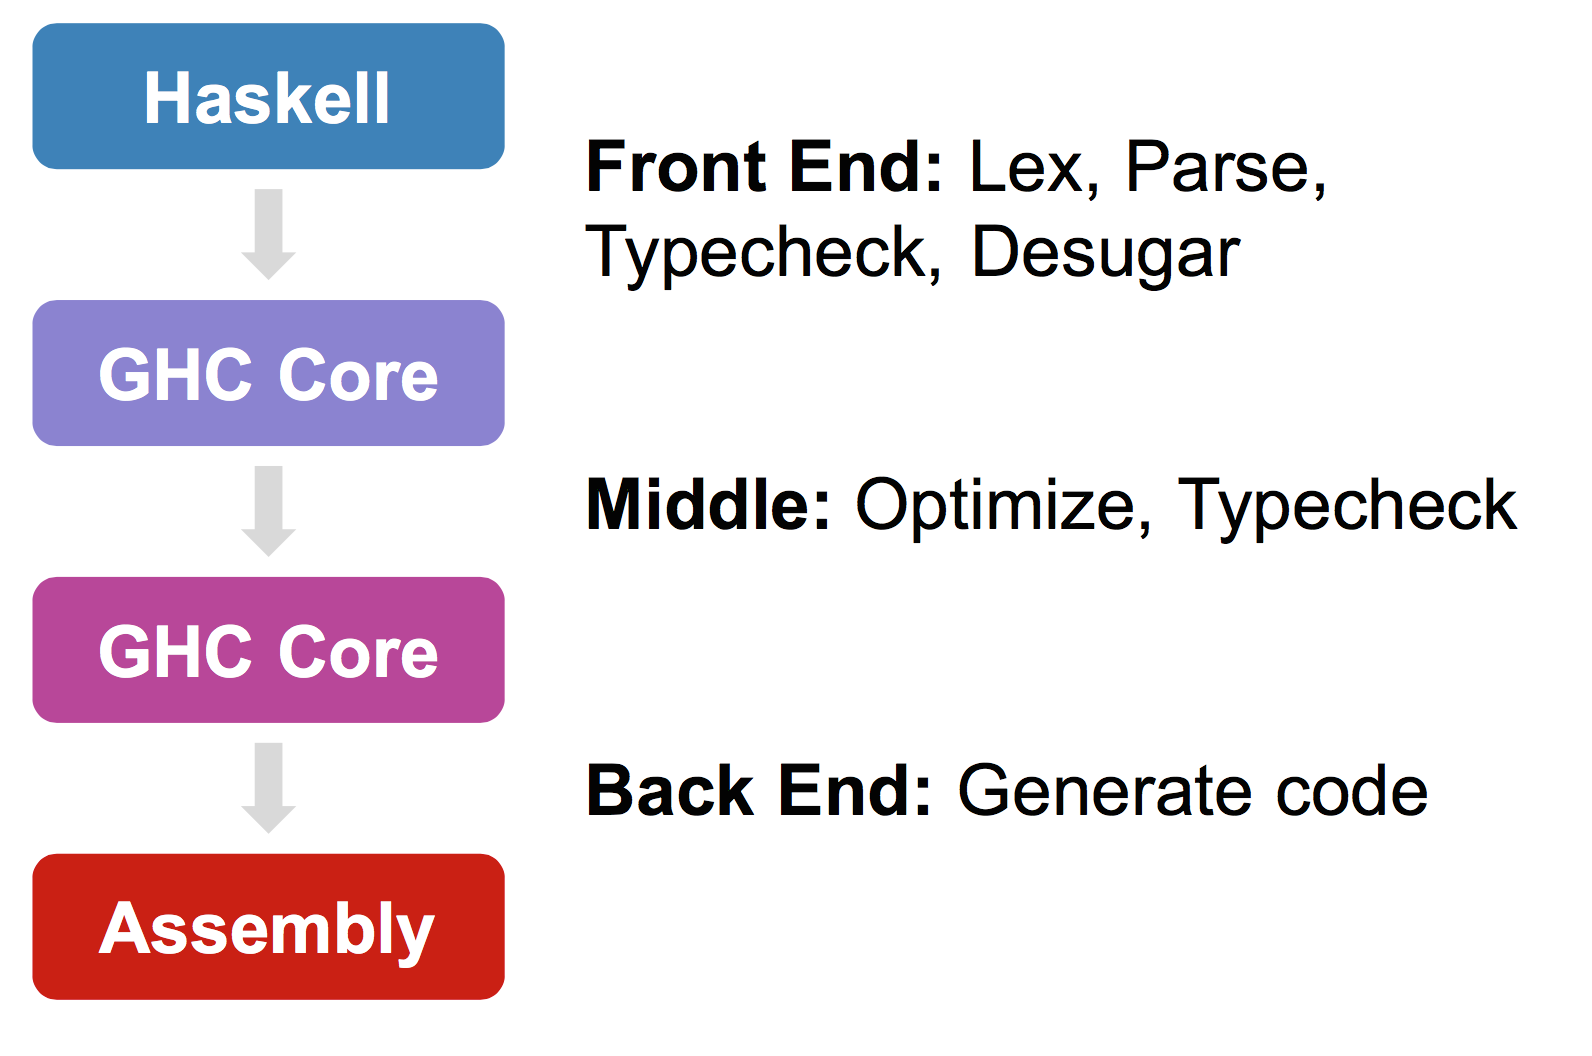
\includegraphics[max width=3in]{desgar.png}
  \caption{The GHC compilation process}
  \label{fig:desgar}
\end{figure}


\subsection{System FC}
\label{sec:background-fc}

(THIS IS ROUGH)

GHC Core is an implementation of System FC, a programming language specification designed for use as a target language for Haskell. System FC is based off the simply typed lambda calculus, an abstract functional language that extends the lambda calculus (consisting of function definitions and function applications) with a constructor for typed functions. 



COERCIONS

\subsection{Type Safety}
\label{sec:background-type-safety}

Should this even be here?!?

\section{Motivation}
\label{sec:motivation}

Content content content

\section{Related Work}
\label{sec:related-work}

Content content content

\section{Implementation}
\label{sec:implementation}

The system is implemented as several Coq modules. These modules each serve a specific purpose. Some of these modules formalize the langauges, others define fixpoint functions for manipulating expressions, and other contains proofs of lemmas and theorems to achieve the full proof.

The formalization of System FC is included in SystemFC.v. This includes formalizations of types, terms, values, and coercions. The formalization follows from the rules for System F from [INSERT TAPL CITATION HERE] and the description of coercions from [INSERT PAPER CITATION HERE]. These rules are formalized in the Coq language through inductive definitions. 

[ How are types defined? ]

[ How are terms defined? ]

[ What are values? ]

[ How are coercions defined? ]

[ Talk about step rules ]

In this formalization of the language, the question of how to model variable naming is addressed. In programming, variables are named with strings, but these can conflict. Conflicting variable names creates a problem for handling shadowing and substitution. For example, when given a function $(\lambda x:Int.\:x + y)$ and attempting to substitute some externally defined variable $x$ for all instances of $y$, problems arise. Performing a na\"ive substitution of $[y \mapsto x] (\lambda x:Int.\:x + y)$ results in a function $\lambda x:Int.\:x + x$. This changes how the function evaluates, so it does not preserve program semantics. Continuing without addressing this source of error in the specification of the operational semantics of the language would make proving the type system to be sound impossible.

There are several ways to get around this substitution issue. The way substitution is handled in the system described is through the use of De Bruijn indices [INSERT DE BRUIJN CITATION HERE]. This means that variables are encoded with natural number values. The value represents the number of binders between the variable's use and its binding site. Given this representation of variables, there cannot be naming conflicts. Consider the following example:
$$\Lambda T.\:\Lambda U.\:\lambda f:T \rightarrow U.\:\lambda x:T.\:f\:x$$
which has type:
$$\forall T.\:\forall U.\:(T \rightarrow U) \rightarrow T \rightarrow U$$
Using De Bruijn indices for both types and terms, the expression becomes:
$$\Lambda.\:\Lambda.\:\lambda : 1 \rightarrow 0.\:\lambda : 1.\:\overline{1}\:\overline{0}$$
which has type:
$$\forall.\:\forall.\:(1 \rightarrow 0) \rightarrow 1 \rightarrow 0$$

Note that the above uses bars to describe identifiers for terms. The $0$ refers to the closest type variable binder and $\overline{0}$ refers to the closest term variable binder. The first expression with traditionally named variables is a simple pair of type abstractions containing a pair of term abstractions related to the types introduced in the outer type abstractions. The variables must be explicitly named at the binding site. This is noted by the $\Lambda T.$ or $\lambda x:T$. Using De Bruijn indices eliminates this need, as referring to a binder just requires determining the distance from the usage site to the binding site. The $\Lambda T.$ in the first example is replaced simply by $\Lambda.$ and the $\lambda x:T$ is transformed into $\lambda : 1$. The $1$ here replaces the $T$, as there is a single type variable binder between the usage of the type and the desired binder.

This representation of variable names using De Bruijn indices is noted in the formalization in SystemFC.v in the variable cases in $ty$, $tm$, and $cn$. All of these definitions take in a natural number as the variable name. This formalization affects the proofs through the rest of the implementation, most notably introducing the need for index shifting. Take, for example, the substitution $[Y \mapsto X] (\Lambda X.\:X \rightarrow Y)$ where $X$ is to be substituted for $Y$ in the type abstraction. Using De Bruijn indices, assume the outer $X$ is known as $2$ and the outer $Y$ is known as $3$ at the binding site outside of the lambda. If this were the case, then the inner $X$ would have to be $0$ using De Bruijn indices, as it refers to the closest binding lambda to it. The inner $Y$ would then refer to the same binder as the outer $Y$. Even though the outer $Y$ is known as $3$ outside of the type abstraction, it must be known as $4$ inside of the abstraction, as an extra binder is introduced between the two uses of $Y$. Despite the confusion this may introduce, this makes the substitution $[3 \mapsto 2] (\Lambda.\:0 \rightarrow 4)$. This is where shifting is relevant. A na\"ive substitution would look for all instances of $3$ and replace them with $2$. This is not correct, though, as the search for uses of $3$ passes a binding site for type variables. This means that what used to be $3$ binders away from the binding site is now $4$ away. Thusly, shifting the index of the substituted variable is necessary to preserve program semantics and adequately work toward a proof of the type safety of System FC.

The fixpoints for shifting types, terms, or coercions are contained in Shifting.v. These shifting functions are used throughout the formalization and proof, most notably through the shifting lemmata contained in SubstProp.v.

The formalization of the evaluation semantics of System FC are defined in Evaluation.v. This includes, most importantly, the step relation. In order to ensure the safety of a type system, some formalization of how expressiosn in the language evaluate is needed to reason about the full execution of a program in the target language. The described formalization takes from the small-step language semantics [CITE SOMEONE HERE] to define how a single expression can take a single step toward its final value. The rules in Evaluation.v form a deterministic relation that is used in defining the major theorems to be proven. These theorems, progress and preservation, rely on the step relation to define how an expression can be evaluated so that they can guaranteed properties about the types at all discrete steps in the program's execution. The theorems for progress, preservation, and soundness are all contained in SystemFCProp.v. This module contains the proof of the type safety of this subset of System FC.

[I'M NOT SURE WHAT TO PUT HERE].

\section{Results}
\label{sec:results}

The system as it stands is a full mechanical proof of the type safety of System F with coercions. The type safety of all features of System FC have previously been proven by hand [CITE THIS], though it has never been done mechanically using a proof assistant. The system described is the first mechanical proof of this particular subset of System FC, namely System F with coercions. Other mechanical proofs of the type safety of System F exist, though none contain a formalization of coercions as described in [CITE SOME PAPER HERE]. 

Given that the Coq interpreter has accepted the proof, it is thought to be verified as a proper proof. The benefits of a mechanical proof over a handwritten one are many in number. A mechanical proof makes use of the Curry-Howard isomorphism to verify the proof instead of relying on the writer and other human verifiers. Beyond just correctness, a mechanical proof is also highly extensible. The system itself is a first for this subset of System FC, but it also allows for further extension to a larger subset, moreso than a handwritten proof could.

[ WHAT EVEN GOES IN THIS SECTION ]

\section{Future Work}
\label{sec:future-work}

As the formalization stands, it does not contain all features commonly thought to be part of System FC. In order to fully match System FC, it would need to be extended to include datatypes and type families. These two additions would create the full formalization of System FC. It would then be necessary to adjust the proofs accordingly so that the Coq interpreter would accept them.

The mechanical proof as it stands is very extensible. This allows for a large number of potential extensions and use cases. Modifying a mechanical proof can be done by adding to an already proper formalization and then walking through the proof with the help of the Coq interpreter. Given that most of the proofs in the system are done by induction on some inductive definition in the formalization, adding to the formalization would add new cases, and much of the proof structure and many of the proofs would be preserved.

Possible future proofs include verifying the safety of various GHC language extensions. GHC includes many features, but programmers are given even more options via extensions to the language. These can be included by annotating the program or including command-line flags to include certain extensions. Many commonly used language extensions add to Haskell's type system, so being able to prove the type safety of an extension would allow for an added level of guarantees to the potentially unsafe extension.

GHC Core is an intermediate representation used in the compilation process of Haskell code. At this level, GHC does many of its optimization passes. Using the formalization and proof of type safety, one could extend the formalization to include a set of optimizations. These optimizations could then be proven to be type safe to ensure the semantics of a program cannot be changed through an invalid optimization done at the GHC Core level.

\section{Ethical Considerations}
\label{sec:ethics}

lol

\section{Conclusion}
\label{sec:conclusion}

Content content content

% We next move onto the bibliography.
\bibliographystyle{plain} % Please do not change the bib-style
\bibliography{final_report}  % Just the *.BIB filename

% Here is a dirty hack. We insert so much vertical space that the
% appendices, which want to begin in the left colunm underneath
% "references", are pushed over to the right-hand column. If we looked
% hard enough, there is probably a command to do exactly this (and
% wouldn't need tweaked after edits).
\vspace{175pt}

\end{document} 
